\chapter{Revisão Bibliográfica} \label{cap2}

\section{Fundamentação Teórica}

\subsection{Estabilidade no Sentido Lyapunov}

% Introdução do teorema de Lyapunov
Os métodos de análise de estabilidade desenvolvidos por Lyapunov são geralmente reconhecidos como base para a compreensão da estabilidade em sistemas dinâmicos. No ano de 1892, o matemático e engenheiro russo, Aleksandr Mikhailovich Lyapunov (1857-1917), propôs abordagens que desempenham um papel crucial na compreensão e caracterização da estabilidade dos sistemas no ponto de equilíbrio. \citep{lyapunov1892}. Em essência, ela se concentra na análise do comportamento das soluções de sistemas dinâmicos em torno de pontos de equilíbrio, estabelecendo critérios para determinar a estabilidade desses pontos, sejam eles estáveis, instáveis ou assintoticamente estáveis. Desta forma, oferece métodos sistemáticos para avaliar a estabilidade de sistemas, tanto autônomos quanto não autônomos, abrangendo desde sistemas lineares até não lineares. \cite{khalil2002}. Ao fornecer condições suficientes para a estabilidade, os métodos de Lyapunov oferecem uma estrutura poderosa para analisar e projetar sistemas dinâmicos com garantias de estabilidade desejadas.

% Bases para o teorema de Lyapunov
Considere o sistema dinâmico representado por \begin{equation}\dot{x} = f(x), \end{equation} onde $f: D \rightarrow \mathbb{R}^n$ é um mapeamento local \textit{Lipschitz} do domínio $D \subset \mathbb{R}^n$ em $\mathbb{R}^n$, e assuma que $\bar{x} \in D$ seja o ponto de equilíbrio do sistema, ou seja, $f(\bar{x}) = 0$. Dada a capacidade de transladar qualquer ponto de equilíbrio para a origem através de mudanças de variáveis, podemos, sem perda de generalização, definir a estabilidade do sistema em relação ao ponto de equilíbrio na origem, ou seja, $\bar{x} = 0$. Assim, podemos apresentar a definição da estabilidade do ponto de equilíbrio, conforme Khalil. \cite{khalil2002}.

\begin{definition}
  O ponto de equilíbrio $\bar{x} = 0$ é

  \begin{enumerate}
    \item[$\bullet$] estável se, para cada $\epsilon > 0$, existe $\delta = \delta(\epsilon) > 0$, tal que,
          $$ \lVert x(0)\rVert < \delta \Rightarrow \lVert x(t)\rVert < \epsilon, \hspace{0.3cm} \forall \, t \geq 0$$
    \item[$\bullet$] instável, se não for estável.
    \item[$\bullet$] assintoticamente estável, se for estável e $\delta$ possa   ser escolhido de forma que:
          $$ \lVert x(0)\rVert < \delta \Rightarrow \lim_{t \rightarrow \infty}x(t) = 0$$
  \end{enumerate}
\end{definition}

Portanto, para demostrar que o ponto de equilíbrio $\bar{x} = 0$ é estável, para qualquer valor de $\epsilon$, deve-se obter um valor de $\delta$, possivelmente dependente de $\epsilon$, de modo que uma trajetória que comece em uma vizinhança $\delta$ da origem nunca sairá da vizinhança $\epsilon$. \cite{khalil2002}.

Khalil, em seu livro \textit{Nonlinear Systems}, demonstrou que a estabilidade do ponto de equilíbrio de um sistema de pêndulo pode ser compreendida através do uso de conceitos de energia. Ele definiu a energia do pêndulo como a soma de suas energias potencial e cinética, com a escolha da referência da energia potencial de modo que a energia do pêndulo na origem seja nula. Ao desconsiderar o atrito, tornando o sistema conservativo e, consequentemente, mantendo a energia do sistema constante, observou-se a formação de um contorno fechado em torno do ponto de origem, especialmente para pequenos valores de energia do sistema. Assim, o ponto de origem é identificado como um ponto de equilíbrio estável. Para sistemas dissipativos, nos quais a energia do sistema diminui ao longo do tempo, ele observou que o sistema converge para a origem conforme o tempo tende ao infinito. Portanto, é possível determinar a estabilidade do ponto de equilíbrio analisando a derivada da função energia ao longo das trajetórias do sistema. \cite{khalil2002}.

Em 1892, Lyapunov afirmou que outras funções, além da energia, podem ser utilizadas para determinar a estabilidade do ponto de equilíbrio. \cite{lyapunov1892}. Dado $V : D \rightarrow \mathbb{R}$ uma função contínua diferenciável definida no domínio $D \subset \mathbb{R}^n$ que contém o ponto de origem. A derivada da função $V$ ao longo da trajetória de $f(x)$, denotado por $\dot{V}(x)$, demostrada por Khalil, \cite{khalil2002}, é dada por: \begin{equation} \dot{V}(x) = \frac{\partial V}{\partial x}f(x). \end{equation} Se $\phi(t;x)$ é a solução de $f(x)$ que inicia no estado inicial $x$ no tempo $t = 0$, então: \begin{equation} \dot{V}(x) = \left. \frac{d}{dt}f(\phi(t;x))\right|_{t=0}. \end{equation} Portanto, se $\dot{V}(x)$ é negativo, $V$ decresce ao longo da solução de $f(x)$.

% Esta é um boa forma de apresentar o teorema?
Com base nos conceitos apresentados até o momento, o teorema de estabilidade de Lyapunov pode ser definido como:

\begin{theorem}[Estabilidade no sentido de Lyapunov \citep{khalil2002}]
  Seja $x = 0$ o ponto de equilíbrio para f(x) e seja $D \subset \mathbb{R}^n$ um domínio contendo $x = 0$. Seja $V : D \rightarrow \mathbb{R}$ uma função diferenciável contínua tal que:
  \begin{gather}
    V(0) = 0 \quad \text{e} \quad V(x) > 0 \quad \mathrm{em} \quad D - \{0\} \label{eq:lyapunov1} \\
    \dot{V}(x) \leq 0 \quad \mathrm{em} \quad D - \{0\} \label{eq:lyapunov2}
  \end{gather}
  Então, $x=0$ é estável. Além disto, se
  \begin{equation}
    \dot{V}(x) < 0 \quad \mathrm{em} \quad D - \{0\} \label{eq:lyapunov3}
  \end{equation}
  então, $x=0$ é assintoticamente estável.
\end{theorem}

%  Definição das função de Lyapunov, superfície de Lyapunov, e função DP e SDP.
Uma função $V(x)$ é chamada de função de Lyapunov quando é contínua e diferenciável, satisfazendo as equações \eqref{eq:lyapunov1} e \eqref{eq:lyapunov2}. A superfície $V(x) = c$, para qualquer $c > 0$, é referida como superfície de Lyapunov. Se $V(x)$ atende à condição \eqref{eq:lyapunov2}, isto é, $V(0) = 0$ e $V(x) > 0$ para $x \neq 0$, ela é considerada definida positiva. No caso em que $V(x)$ satisfaz $V(x) \geq 0$ para $x \neq 0$, ela é denominada semidefinida positiva. Uma função $V(x)$ é classificada como definida negativa ou semidefinida negativa se $-V(a)$ é definida positiva ou semidefinida positiva, respectivamente. Se $V(x)$ não se enquadra em nenhum desses casos, é considerada indefinida. Com essa terminologia, o teorema de Lyapunov pode ser reformulado, indicando que a origem é estável se existe uma função $V(x)$ definida positiva, continuamente diferenciável, tal que $\dot{V}(x)$ seja semidefinida negativa. Além disso, a estabilidade assintótica é alcançada quando $\dot{V}(x)$ é definida negativa. \cite{khalil2002}.

%  Definição das Matrizes SDP E DP
Uma classe de funções escalares para as quais a determinação do sinal pode ser facilmente realizada é a classe das funções quadráticas, representadas por:

\begin{equation}
  V(x) = x^T P x = \sum_{i=1}^n \sum_{j=1}^n p_{ij} x_i x_j
  \label{eq:lyapunov4}
\end{equation}

\noindent onde $P$ é uma matriz real simétrica. Nesse caso, $V(x)$ é positiva definida ou positiva semidefinida se, e somente se, todos os autovalores de $P$ são positivos ou não negativos, o que ocorre se e somente se todos os menores principais de $P$ são positivos ou não negativos, respectivamente. Se $V(x) = x^T P x$ é positiva definida ou positiva semidefinida, dizemos que a matriz $P$ é positiva definida ou positiva semidefinida, representado por $P > 0$ ou $P \geq 0$, respectivamente. \cite{khalil2002}.

%  To-do: adicionar um conclusão e uma ponte para LMIs
\subsection{Desigualdades Matriciais Lineares}

% Introdução às LMIs
As desigualdades matriciais lineares (\acrshortpl{lmi}, do inglês \textit{Linear Matrix Inequalities}) são de grande importância na teoria de controle e sistemas, fornecendo uma estrutura significativa para a formulação e resolução de uma variedade de problemas. Este conjunto de técnicas permite a representação de restrições complexas em termos de desigualdades lineares entre matrizes, possibilitando a abordagem de questões como estabilidade, desempenho e síntese de controladores de forma unificada. \cite{boyd1994}.

Os métodos de Lyapunov tradicionalmente empregados na análise de estabilidade de sistemas dinâmicos têm sido estendidos para permitir a formulação de \acrshortpl{lmi}, proporcionando assim uma base teórica sólida para a resolução de problemas de otimização e controle. Essa conexão entre \acrshortpl{lmi} e Lyapunov não apenas simplifica a análise e a síntese de sistemas complexos, mas também oferece uma estrutura matemática para abordar uma variedade de questões de controle de forma eficiente e sistemática. \cite{boyd1994}.

% História das LMIs
Como discutido na seção anterior, Lyapunov introduziu seus teoremas, estabelecendo que um sistema dinâmico \begin{equation} \dot{x}(t) = Ax(t) \label{eq:sys1}\end{equation} é assintoticamente estável se, e somente se, as condições descritas nas equações \eqref{eq:lyapunov1} e \eqref{eq:lyapunov3} forem satisfeitas. Adicionalmente, ele propôs uma classe de funções de Lyapunov que atendem a essas condições, conforme apresentado na equação \eqref{eq:lyapunov4}. Substituindo esta equação nas condições de estabilidade, obtemos: \begin{equation} \dot{V}(x) = \dot{x}^TPx + x^TP\dot{x} \label{eq:lyapunov5}. \end{equation} A partir do sistema (\ref{eq:sys1}), a equação (\ref{eq:lyapunov5}) pode ser reescrita como: \begin{equation} \dot{V}(x) = x^TA^TPx + x^TPAx \label{eq:lyapunov6}. \end{equation} logo, \begin{equation} \dot{V}(x) = x^T (A^TP + PA) x \label{eq:lyapunov6}, \end{equation} ou seja, o sistema (\ref{eq:sys1}) é assintoticamente estável se, e somente se, existir uma matriz definida positiva $P$ tal que \begin{equation} A^T P + P A < 0.\end{equation}

Essa condição, conhecida como desigualdade de Lyapunov em $P$, é uma forma específica de \acrshort{lmi}. Lyapunov também demonstrou que essa LMI inicial poderia ser resolvida explicitamente. Na prática, é possível escolher qualquer $Q = Q^T > 0$ e resolver a equação linear $A^T P + P A = -Q$ para a matriz $P$. Se o sistema for estável, a matriz $P$ resultante será definida positiva. Assim, a desigualdade de Lyapunov foi a primeira \acrshort{lmi} utilizada para analisar a estabilidade de sistemas dinâmicos, oferecendo uma solução analítica por meio da resolução de um conjunto de equações lineares. \cite{lyapunov1892,boyd1994}.

Após os trabalhos iniciais de Lyapunov, na década de 1940, pesquisadores soviéticos como Lur'e e Postnikov aplicaram seus métodos em problemas práticos de controle, focando especialmente na estabilidade de sistemas com não-linearidades nos atuadores. Embora suas soluções fossem resolvidas manualmente e aplicáveis apenas a sistemas menores, esse trabalho foi crucial para demonstrar a viabilidade das ideias de Lyapunov na engenharia de controle. O avanço seguinte, nos anos 1960, trouxe métodos gráficos mais acessíveis, expandindo o alcance para sistemas mais complexos e estabelecendo as bases para a resolução computacional das LMIs, marcando assim uma nova fase na teoria do controle. \cite{boyd1994}.

% Definição de um LMI
A seguir, é apresentado o conceito formal de uma \acrshort{lmi}, conforme definido por Boyd et al. \cite{boyd1994}.

\begin{definition}
  Uma \acrshort{lmi} é expressa pela equação \begin{equation} F(x) \triangleq F_0 + \sum_{i=0}^{m}(x_iF_i) > 0 \label{eq:lmi1}\end{equation} onde $x \in \mathbb{R}^m$ é a variável e as matrizes simétricas $F_i \in \mathbb{R}^{n \times n}, \, i = 0, . . . , m$, são fornecidas. Nesta expressão, o símbolo de desigualdade indica que $F(x)$ é definida positiva. Além disso, há \acrshortpl{lmi} não estritas, representadas pela forma \begin{equation} F(x) \geq 0 \end{equation}
\end{definition}

Múltiplas \acrshortpl{lmi}  $F_{(1)}(x) > 0, \, ..., \, F_{(p)}(x) > 0$ podem ser expressas como uma única \acrshort{lmi} $\mathbf{diag}(F_{(1)}(x), \, ..., \, F_{(p)}(x)) > 0$. Além disto, quando as matrizes $F_i$ são diagonais, a LMI $F(x) > 0$ é apenas um conjunto de desigualdades lineares. As desigualdades não lineares (convexas) são convertidas para a forma LMI usando complementos de Schur.

A \acrshort{lmi} \eqref{eq:lmi1} é uma restrição convexa em $x$, tornando o conjunto $\{x \, : \, F(x) > 0\}$ convexo e pode representar uma ampla variedade de restrições convexas em $x$, incluindo desigualdades lineares, quadráticas, de norma de matriz, bem como restrições comuns em teoria de controle, como desigualdades matriciais quadráticas convexas e de Lyapunov. \cite{boyd1994}.

\subsection{Sistemas de Controle Baseado em Eventos} \label{subsection:etc}

% ETC: Introdução
O \acrfull{etc}, surgindo como uma solução, se destaca em \acrfullpl{scr}, onde conectam componentes como sensores, controladores e atuadores através de uma rede compartilhada. Enquanto os \acrshortpl{scr} geralmente adotam o controle periódico, o que pode causar congestionamentos e desperdícios de recursos, o \acrshort{etc} executa tarefas apenas quando necessárias, minimizando estes problemas. Ele pode ser modelado de diversas formas, com destaque para o modelo de atraso de tempo, que permite lidar com atrasos de transmissão e otimizar ganhos de controle. Esses modelos despertam interesse entre pesquisadores, especialmente em estudos de estabilidade e design de controladores \citep{peng2018}.

\subsubsection{Sistemas dinâmicos em malha fechada sob \acrshort{etc}}
O modelo de um sistema dinâmico em malha fechado sob um \acrshort{etc} pode ser descrito como um modelo típico de controle por realimentação de estados, conforme ilustrado na figura a seguir:

\begin{figure}[H]
  \centering
  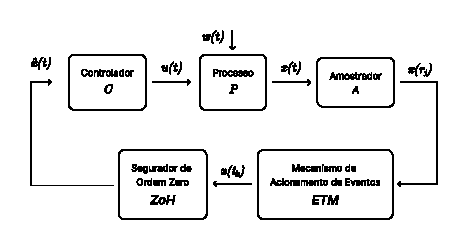
\includegraphics[width=0.87\textwidth]{figuras/etc-model.eps}
  \caption{Modelo de um sistema dinâmico em malha fechada com ETC.}
  \label{fig:closed_loop_etc}
\end{figure}

% ETC: Estrutura
O modelo apresentado na \autoref{fig:closed_loop_etc} consiste em uma planta $P$ que recebe uma entrada de perturbação não controlada $w(t)$ e a entrada de controle $u(t)$, e cujo estado é determinado por uma equação diferencial expressa por: \begin{equation}\dt{x}(t) = f(x(t), u(t), w(t))\end{equation} A informação do estado pode ser monitorada de forma contínua ou amostrada, o que caracteriza o \acrshort{etc} como contínuo ou periódico, respectivamente. No caso do \acrshort{etc} periódico, um sistema de amostragem é introduzido para gerar uma sequência discreta de estados $x(t_r)$, onde o $t_r$ é o tempo de liberação do estado medido. Por outro lado, no \acrshort{etc} contínuo, o estado medido é enviado diretamente para o \acrshort{etm} \citep{peng2018,coutinho2021,Lemmon2010}.

% ETC: Função do ETM e comportamento Zeno
O \acrshort{etm} determina o instante apropriado para transmitir o estado para o \acrfull{zoh} - que é utilizado para transformar o sinal discreto resultante em um sinal contínuo no tempo para estar disponível para o controlador $C$, que por sua vez irá mapear esses estados transmitidos em um sinal de controle e aplicar à planta por meio da seguinte lei de controle por realimentação de estados: \begin{equation}u(t) = K \hat{x}(t),\end{equation} onde $\hat{x}$ representa o último estado disponível para o controlador \citep{coutinho2021}. Para garantir a eficácia do \acrshort{etm}, é crucial evitar o comportamento Zeno. Esse comportamento ocorre quando o controlador executa uma quantidade infinita de tarefas de controle dentro de um intervalo de tempo finito, contrariando a premissa fundamental do \acrshort{etc} de minimizar a quantidade de tarefas a serem executadas. Além disso, o fenômeno de Zeno exerce uma considerável influência nos comportamentos dinâmicos dos sistemas, manifestando-se em instabilidade, degradação de desempenho e oscilações indesejadas \citep{Yang2024}.

% ETC: Rede de Comunicação
Os efeitos induzidos aos estados transmitidos pela rede de comunicação $\mathcal{N}$ são de suma importância e têm um impacto direto na estabilidade e no desempenho do sistema. Quando os estados são transmitidos por meio da rede, podem surgir distorções e atrasos devido a vários fatores, como variações nos intervalos de transmissão, atrasos na própria rede e possíveis perdas de pacotes. Essas perturbações nos estados transmitidos podem resultar em erros na estimativa do estado real no controlador, afetando diretamente a capacidade do sistema de alcançar os objetivos de controle desejados. Assim, é essencial compreender e mitigar esses efeitos nos estados transmitidos para garantir um projeto eficaz dos controladores, o que por sua vez assegura a estabilidade e o desempenho adequados do sistema em malha fechada \citep{coutinho2021}.

% % ETC: Conclusão
% As diferentes abordagem de \acrshort{etc} abrangem investigações em controladores de retroalimentação de estado, observadores, \acrshortpl{etm} estáticos e dinâmicos, com o intuito de assegurar a estabilidade e o desempenho em malha fechada em uma variedade de sistemas, tais como sistemas \acrfullpl{lit} \cite{Zong2023,Wu2021}, sistemas de \textit{Lur'e} \cite{Zhang2017} e modelos \textit{fuzzy Takagi-Sugeno} \cite{Pan2017}. O foco está em estabelecer condições práticas e numericamente solucionáveis que simplifiquem o projeto eficaz de sistemas de controle complexos.

% ---------------------------------------------------------------------------
\subsubsection{\acrshort{etm} estático, adaptativo e dinâmico} \label{section:etm_classification}

% ETM dinâmico e estático: introdução
Os modelos de \acrshort{etm} podem ser classificados com base na sua lei de acionamento de eventos, que pode ser estática ou dinâmica. No contexto do ETM estático e do modelo apresentado na \autoref{fig:closed_loop_etc}, o acionamento dos eventos de transmissão de novos dados é determinado por uma função de evento estática representada por: \begin{equation}
  \Gamma(x(t), \hat{x}(t)) \label{eq:static_gamma_function_1}
\end{equation} Isso implica que o \acrshort{etm} estático depende apenas dos estados atuais ($x$) do sistema e dos estados transmitidos anteriormente ($\hat{x}$).

% ETM dinâmico e estático: estabilidade do sistema sob ETM estático
A estabilidade assintótica do sistema em malha fechada sob um \acrshort{etm} estático é garantida se existir uma função de Lyapunov $V(x)$ que satisfaça as seguintes condições: \begin{gather}
  \alpha_1(\| x(t) \|) \leq V(x) \leq \alpha_2(\| x(t) \|) \label{eq:static_etm_v} \\[8pt]
  \dot{V}(x) \leq - \alpha(\|x(t)\|) + \beta(\|e(t)\|), \label{eq:static_etm_dot_v_1}
\end{gather} onde $ \alpha_1 , \, \alpha_2, \, \alpha, \, \beta \in \mathcal{K}_\infty $ e \begin{equation}
  e(t) = x(t) - \hat{x}(t).
\end{equation} Assim, é possível definir uma função de evento estática $ \Gamma(x(t), \hat{x}(t)) $ da seguinte forma: \begin{equation}
  \Gamma(x(t), \hat{x}(t)) = \sigma \alpha(\|x(t)\|)- \beta(\|x(t) - \hat{x}(t)\|),
\end{equation} ou, em termos de $e(t)$, \begin{equation}
  \Gamma(x(t), e(t)) = \sigma \alpha(\|x(t)\|)- \beta(\|e(t)\|),
  \label{eq:static_gamma_function_2}
\end{equation} 
para $ \sigma \in (0, 1) $. Além disso, os instantes de acionamento de novos eventos de transmissão são determinados quando a função de evento $\Gamma$ for negativa, ou seja, \begin{equation}
  t_0 = 0, \, t_{k+1} = \inf\{t > t_k, \, \Gamma(x, e) < 0\}, \, \forall k \in \mathbb{N}. \label{eq:static_event_triggering_law}
\end{equation} Esta expressão, \eqref{eq:static_event_triggering_law}, é a lei de acionamento de eventos do \acrshort{etm} estático. 

Desta forma, enquanto não ocorrer uma nova transmissão, ou seja, $\Gamma \geq 0$, tem-se: \begin{gather}
  \sigma \alpha(\|x(t)\|)- \beta(\|e(t)\|) \geq 0 \\[8pt]
  \beta(\|e(t)\|) \leq \sigma \alpha(\|x(t)\|). \label{eq:alpha_beta_condition}
\end{gather} Portanto, a partir da condições descritas em \eqref{eq:static_etm_dot_v_1} e \eqref{eq:alpha_beta_condition}, obtém-se: \begin{gather}
  \dot{V}(x) \leq - \alpha(\|x(t)\|) - \sigma \alpha(\|x(t)\|) < 0, \\[8pt]
  \dot{V}(x) \leq - (1 - \sigma)\alpha(\|x(t)\|) < 0, \label{eq:static_etm_dot_v_2}
\end{gather} garantindo que o sistema seja assintoticamente estável sob o \acrshort{etm} estático.

% ETM dinâmico e estático: variáveis dinâmicas e ETM adaptativo
Para reduzir o número de transmissões, foram propostas funções de acionamento aprimoradas \citep{Wang2020,Zong2023,Ge2017, Ning2018, Wu2021}, por meio da adição de variáveis dinâmicas ao \acrshort{etm} estático, classificando-o em adaptativo ou dinâmico. No \acrshort{etm} adaptativo, o comportamento dinâmico é obtido ao considerar $\sigma$ como uma variável dinâmica, em contraste à sua versão no \acrshort{etm} estático. Assim sendo, a função de eventos $\Gamma$ para o \acrshort{etm} adaptativo pode ser definida como: \begin{equation}
  \Gamma(x(t), e(t), \sigma(t)) = \sigma \alpha(\|x(t)\|)- \beta(\|e(t)\|),
  \label{eq:adaptative_gamma_function_2}
\end{equation} onde \begin{equation}
  \dt{\sigma} = \Omega(\sigma(t), e(t)),
\end{equation} com o valor inicial $\sigma(0) \in (0, 1)$. Além disto, a função $\Omega$ geralmente é definida como: \begin{equation}
  \Omega(\sigma(t), e(t)) = \frac{1}{\sigma}\left(\frac{1}{\sigma} - \sigma_0\right)\beta(\|e(t)\|), \label{eq:omega_function}
\end{equation} onde $\sigma_0$ é um parâmetro de projeto.

% ETM dinâmico e estático: estabilidade sob ETM adaptativo
Para análise da estabilidade assintótica de um sistema em malha fechada sob um \acrshort{etm} adaptativo, considera-se uma função de Lyapunov $W(x)$ definida como: \begin{equation}
  W(x(t), \sigma(t)) = V(x(t)) + \frac{1}{2}\sigma^2(t),
\end{equation} onde $V(x)$ é a função de Lyapunov apresentada em \eqref{eq:static_etm_v}. Assim, a partir das condições \eqref{eq:static_etm_dot_v_1} e \eqref{eq:omega_function}, pode-se determinar a derivada temporal de $W$ como: \begin{gather}
  \dot{W}(x(t), \sigma(t)) = \dot{V}(x(t)) + \sigma(t) \dot{\sigma}(t) \\[8pt]
  \dot{W}(x(t), \sigma(t)) \leq - \alpha(\|x(t)\|) + \beta(\|e(t)\|) + \left(\frac{1}{\sigma(t)} - \sigma_0\right)\beta(\|e(t)\|).
\end{gather} Da mesma forma que foi estabelecido no \acrshort{etm} estático, um evento somente é acionado quando a função de evento $\Gamma$ for negativa. Consequentemente, a lei de acionamento do \acrshort{etm} adaptativo é definida como: \begin{equation}
  t_0 = 0, \, t_{k+1} = \inf\{t > t_k, \, \Gamma(x, e, \sigma) < 0\}, \, \forall k \in \mathbb{N}. \label{eq:adaptative_event_triggering_law}
\end{equation} Portanto, enquanto não ocorrer uma nova transmissão, a condição apresentada em \eqref{eq:alpha_beta_condition} será satisfeita. Logo, \begin{gather}
  \dot{W}(x(t), \sigma(t)) \leq - \alpha(\|x(t)\|) - \sigma \alpha(\|x(t)\|) + \left(\frac{1}{\sigma(t)} - \sigma_0\right)\beta(\|e(t)\|) < 0, \\[8pt]
  \dot{W}(x(t), \sigma(t)) \leq - \alpha(\|x(t)\|) - \sigma \alpha(\|x(t)\|) + \left(\frac{1}{\sigma} - \sigma_0\right) (- \sigma \alpha(\|x(t)\|)) < 0, \\[8pt]
  \dot{W}(x(t), \sigma(t)) \leq - \sigma(t)(\sigma_0 - 1) \alpha(\|x(t)\|) < 0,
\end{gather} garantindo a estabilidade assintótica do sistema em malha fechada sob o \acrshort{etm} adaptativo.

% ETM dinâmico e estático: ETM dinâmico
No \acrshort{etm} dinâmico, a variável dinâmica é incorporada diretamente na lei de acionamento do \acrshort{etm} estático. Enquanto no ETM estático e no adaptativo, o evento de transmissão era acionado quando a função-evento $\Gamma$ se tornava negativa, no ETM dinâmico, este acionamento é determinado quando a seguinte expressão é negativa: \begin{equation}
  \eta(t) + \theta\Gamma(x(t), e(t)),
\end{equation} onde $\Gamma(x, e)$ é a função-evento definida para o ETM estático em \eqref{eq:static_gamma_function_2}, $\theta$ é um parâmetro de projeto e $\eta(t) \in \mathbb{R}_{\geq 0}$ é a variável dinâmica expressa por: \begin{equation}
  \dt{\eta}(t) = \delta(\eta(t)) + \sigma \alpha(\|x(t)\|) - \beta(\|e(t)\|).
  \label{eq:dynamic_etm_dot_eta}
\end{equation} onde o seu valor inicial $\eta(0) = \eta_0 \in \mathbb{R}_{\geq 0}$, $\delta \in \mathcal{K}_\infty$ e os parâmetros $\sigma$, $\alpha$ e $\beta$ definidas anteriormente. Por consequência, a lei de acionamento do \acrshort{etm} dinâmico é descrita por: \begin{equation}
  t_0 = 0, \, t_{k+1} = \inf\{t > t_k, \, \eta(t) + \theta \Gamma(x, e) < 0\}, \, \forall k \in \mathbb{N}. \label{eq:dynamic_event_triggering_law}
\end{equation}

% ETM dinâmico e estático: ETM dinâmico vs ETM estático
A variável dinâmica $\eta(t)$ age como um filtro da função de acionamento do ETM estático. Sua principal vantagem sobre o ETM estático é a capacidade de manter o mesmo desempenho em malha fechada, exigindo menos eventos transmitidos e, portanto, menos recursos de comunicação. Além disso, o próximo tempo de transmissão no ETM dinâmico é igual ou maior que no ETM estático, o que implica na existência de um \acrshort{imee} positivo, se tal \acrshort{imee} existir para a versão estática do ETM em estudo \citep{coutinho2021}.

% ETM dinâmico e estático: estabilidade sob ETM dinâmico
Para análise da estabilidade assintótica de um sistema em malha fechada sob um \acrshort{etm} dinâmico, considera-se uma função de Lyapunov $W(x)$ definida como: \begin{equation}
  W(x, \eta) = V(x) + \eta,
\end{equation} onde $V(x)$ é a função de Lyapunov apresentada em \eqref{eq:static_etm_v}. Desta forma, a derivada temporal de $W$ é definida como: \begin{equation}
  \dt{W}(x(t), \eta(t)) = \dt{V}(x(t)) + \dt{\eta}(t).
\end{equation} A partir da condição \eqref{eq:static_etm_dot_v_1} e da equação dinâmica de $\eta(t)$ definida em \eqref{eq:dynamic_etm_dot_eta}, obtém-se: \begin{gather}
  \dt{W}(x(t), \eta(t)) \leq - \alpha(\|x(t)\|) + \beta(\|e(t)\|) + \delta(\eta(t)) + \sigma \alpha(\|x(t)\|) - \beta(\|e(t)\|) < 0\\[8pt]
  \dt{W}(x(t), \eta(t)) \leq - (1 - \sigma)\alpha(\|x(t)\|) - \delta(\eta(t)) < 0.
\end{gather} Portanto, a estabilidade assintótica é garantida para um sistema operando sob o ETM dinâmico.

% ---------------------------------------------------------------------------
\subsubsection{Abordagens de projeto do \acrshort{etm}}

% ETC: Diferentes Abordagens - Introdução
Para assegurar o desempenho adequado e a estabilidade dos sistemas sob o \acrshort{etc} em malha fechada, é crucial o projeto eficiente tanto do \acrshort{etm} quanto das leis de controle. Como resultado, os modelos de \acrshort{etc} frequentemente adotam abordagens baseadas em emulação ou co-design para atingir tais objetivos \citep{coutinho2021, peng2018}. 

% ETC: Diferentes Abordagens - Abordagem por Emulação
As abordagens baseadas em emulação são geralmente realizadas em dois passos distintos. Primeiramente, um controlador é projetado para garantir a estabilidade ou um desempenho específico para o sistema em malha fechada, assumindo a ausência do \acrshort{etm} e da rede de comunicação. Este controle é projetado de acordo com uma estrutura convencional de dados amostrados periódicos, aproveitando os resultados proveitosos dos sistemas de dados amostrados \citep{coutinho2021,peng2018}. O próximo passo envolve considerar a presença do \acrshort{etm} e os efeitos induzidos pela rede de comunicação, a fim de projetar o \acrshort{etm} de forma a preservar as propriedades garantidas pelo controlador previamente projetado. Esta abordagem permite que o \acrshort{etm} seja projetado separadamente do controle, conferindo flexibilidade no processo de projeto \citep{coutinho2021,peng2018}. No entanto, essa independência pode limitar o desempenho em malha fechada do sistema \acrshort{etc} e exigir mais transmissões do que o necessário, uma vez que o \acrshort{etm} pode não estar otimizado para o controle específico \citep{coutinho2021}.

% ETC: Diferentes Abordagens - Abordagem por Co-design
As abordagens baseados no co-design buscam superar as limitações das abordagens baseadas em emulação, permitindo o projeto simultâneo do \acrshort{etm} e da lei de controle. No entanto, o co-design enfrenta desafios como problemas de otimização não-convexos ou multiobjetivo, devido a restrições conflitantes de desempenho e aumento dos tempos entre eventos \cite{coutinho2021}. Diferentes estratégias de co-design têm sido desenvolvidas para várias formas de \acrshortpl{etm}. Estas incluem co-design estático para estabilização local de sistemas \acrshortpl{lit} e co-design dinâmico para sistemas lineares com entradas não lineares limitadas, entre outros. As condições de co-design são frequentemente derivadas usando formalismos de sistema híbrido e expressas em termos de \acrshortpl{lmi}, permitindo uma eficiente resolução por métodos de otimização convexa \cite{coutinho2021}.

\section{Trabalhos relacionados}

A área de sistemas \acrshort{etc} já possui diversas técnicas estabelecidas que têm demonstrado resultados promissores. As estratégias adotadas neste projeto têm sua base em pesquisas destacadas que serão apresentadas a seguir

% To-do: Explicar sobre o comportamento Zeno na fundamentação
% Dúvida: É para ser mais detalhistas em cada trabalho?
Em sua pesquisa, \cite{coutinho2021} investigou sobre um modelo de \acrshort{etm} dinâmico e estático, sobre o qual este projeto se fundamenta. Esse modelo permite o projeto simultâneo do \acrshort{etm} e do controlador, utilizando a abordagem de co-design para garantir a estabilidade do sistema em malha fechada. O estudo também demonstra a existência de um \acrfull{imee} positivo para evitar comportamento de Zeno, tornando-o aplicável em redes de comunicação com largura de banda finita. Por fim, ele aborda otimização para ampliar os intervalos entre eventos, visando minimizar a quantidade de eventos gerados pelo \acrshort{etm}.

% Lembrete: Este trabalho apresenta a definição de zoh
% Dúvida: Há um termo melhor para 'switched systems'?
\textit{Ren et al}. \cite{Ren2018} abordaram o controle resiliente de tempo finito com base em observadores para sistemas comutados, realizado em um \acrfull{ecae}. Diferenciando-se dos problemas tradicionais de tempo finito, este estudo considera não apenas o \acrfull{ltf}, mas também a \acrfull{efes}. Um \acrshort{ecae} é formulado para sistemas comutados, visando uma utilização eficiente dos recursos da rede. Para lidar com a impossibilidade de medir todos os estados, é desenvolvido um observador acionado por eventos, que serve como base para a construção de um controlador resiliente. Esse controlador demonstra robustez ao estabilizar os sistemas em questão, dentro do contexto do controle de tempo finito. Utilizando o método de atraso no tempo e a abordagem de Lyapunov, são derivados resultados significativos para avaliar as propriedades dos \acrshortpl{ltf} e da \acrshort{efes} dos sistemas de erro comutados em circuito fechado acionados por eventos. Todas as desigualdades matriciais são transformadas em \acrshortpl{lmi} para facilitar a obtenção conjunta dos ganhos do controlador e do observador. Por fim, a eficácia do esquema de controle proposto é demonstrada através de sua aplicação em um sistema de circuito de conversor \textit{boost}.

No estudo apresentado por \textit{Soni et al}. \cite{Soni2023}, é proposto o \acrshort{etc} para o modelo \acrshort{lpv} de conversores \textit{boost}. O controlador proposto, dependente da razão de ciclo, demonstra melhor desempenho e menor demanda computacional. Utilizando a função de \textit{Lyapunov } dependente de parâmetros, foi realizada a análise de estabilidade da abordagem proposta. Além disso, é estabelecido que o tempo entre eventos é limitado inferiormente por uma constante positiva, assegurando um desempenho livre de comportamento \textit{Zeno}. Os resultados de simulação e experimentais deste estudo validam a eficácia do método proposto, evidenciando que o modelo proporciona desempenho e maior robustez.

% Dúvida: Há um termo melhor para 'switched systems'?
No estudo realizado por Ma et al. \cite{Ma2016}, o problema do \acrshort{etc} com base em retroalimentação de saída para sistemas lineares comutados é investigado. Os autores projetam um controlador acionado por eventos e derivam condições suficientes para garantir a estabilidade assintótica do sistema comutado, utilizando métodos da função de Lyapunov e técnicas de \acrshortpl{lmi}. Além disso, eles demonstram que o \acrshort{imee} acionados é positivo, eliminando o comportamento Zeno na amostragem. Por fim, os pesquisadores aplicam seu método a sistemas comutados de conversores \textit{boost} para validar sua eficácia.

\textit{Xie et al.} \cite{Xie2023} abordam os problemas da análise de \acrshort{efes} e do projeto de controlador de retroalimentação de saída para sistemas afins comutados sujeitos a perturbações externas. Um observador afim comutado é desenvolvido para estimar estados não mensuráveis, seguido pela proposição de um \acrshort{etm} dinâmico capaz de evitar o comportamento Zeno e reduz a carga de transmissão da rede. As condições viáveis da \acrshort{ees} são apresentadas em formas de \acrshortpl{lmi}, baseadas em uma função de \textit{Lyapunov-Krasovskii} temporal e leis de comutação dependentes do estado. A eficácia do algoritmo proposto é demonstrada através de um exemplo de aplicação com um conversor \textit{flyback} CC-CC.

No artigo \cite{Kumar2020}, Kumar et al. introduzem um novo conceito de \acrshort{etc} para otimizar o uso de recursos em \acrshort{mgcc}. Um \acrfull{cmd} é combinado com um observador de perturbações integral para suprimir incertezas combinadas e não combinadas em modo conectado à rede e isolado. O controlador resultante regula a tensão do barramento \acrshort{cc} e melhora a estabilidade operacional da \acrshort{mr}. Um \acrshort{cmd} convergente em tempo finito, livre de oscilações, é desenvolvido com uma lei de alcance de super torção para garantir robustez. A eficácia do \acrshort{etc} é comparada com abordagens alternativas e demonstrou um desempenho superior.
